\documentclass{standalone}
%-----------------------------------------------------------------------------%
%%% Color %%%
\usepackage{xcolor}
\definecolor{myred}{RGB}{229,0,0}
\definecolor{myblue}{RGB}{0,98,144}
\definecolor{myyellow}{RGB}{246,182,50}
\definecolor{mygreen}{RGB}{75,108,89}
\newcommand{\red}[1]{\textcolor{myred}{#1}}
\newcommand{\blue}[1]{\textcolor{myblue}{#1}}
\newcommand{\yellow}[1]{\textcolor{myyellow}{#1}}
%-----------------------------------------------------------------------------%
%%% TikZ %%%
\usepackage{tikz}
% \usetikzlibrary{calc}
% \usetikzlibrary{positioning}
% \usetikzlibrary{patterns}
% \usetikzlibrary{fit}
% \usetikzlibrary{angles,quotes}
% \usetikzlibrary{intersections}
% \usetikzlibrary{decorations.markings}
%-----------------------------------------------------------------------------%

\begin{document}

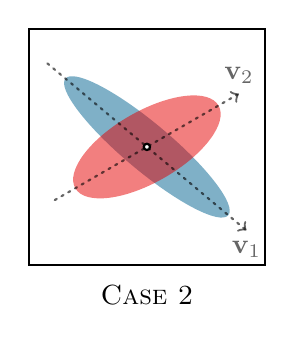
\begin{tikzpicture}[scale=1.5,thick,line cap=round]
	\tikzstyle{jiao}=[solid,circle,draw,fill=white,inner sep=.8pt];
	\draw[draw=none,rotate=50,opacity=0.50,fill=myblue] (0,0) ellipse (0.2cm and 0.9cm);
	\draw[draw=none,rotate=30,opacity=0.50,fill=myred]  (0,0) ellipse (0.7cm and 0.3cm);
	\draw[dotted,->,opacity=0.6] (140:1.1) -- (-40:1.1) node[below]{$\mathbf{v}_1$};
	\draw[dotted,->,opacity=0.6] (210:0.9) -- (30:0.9)  node[above]{$\mathbf{v}_2$};
	\draw (-1,-1) rectangle (1,1);
	\node[jiao] at (0,0) {};
	\node[label=below:{\textsc{Case 2}}] at (0,-1) {};
\end{tikzpicture}

\end{document}
